%%%%%%%%%%%%%%%%%%%%%%%%%%%%%%%%%%%%%%%%%%%%%%%%%%%%%%%%%%%%%%%%%%%%%%
%% <3 Ninjas in Pyjamas <3
%%%%%%%%%%%%%%%%%%%%%%%%%%%%%%%%%%%%%%%%%%%%%%%%%%%%%%%%%%%%%%%%%%%%%%
%

\documentclass[12pt]{article}
\usepackage{float}
\usepackage[bottom]{footmisc}
\usepackage{cite}
\usepackage{graphicx}
\usepackage{longtable}
\graphicspath{{figures/}} % Graphics will be here
\usepackage[utf8]{inputenc}
\usepackage[T1]{fontenc}
\usepackage{listings}
%
% Pagestyle
%
\oddsidemargin9.6mm
\evensidemargin9.6mm
\topmargin-1cm
\headheight20pt
\textwidth155mm
\textheight232mm
\pagestyle{myheadings}
%
% Macros
%
\newcommand\fbe{{\tt fbe\_tez}}
\newcommand\report{{\tt report}}
\newcommand{\bq}{\begin{quotation}\noindent}
\newcommand{\eq}{\end{quotation}}
\renewcommand{\arg}[1]{$\langle\mbox{\it #1}\rangle$}
%
% Title declarations
%

\title{{\Huge CmpE 443 Final Project Report } \\ Group Name : Ninjas in Pyjamas(NIP)  }
\author{Members \\ Faik Emre Derin(Team Leader) \\ Huriye Özdemir\\ Özge Dinçsoy \\ Ergün Erdoğmuş}
\date{December 29, 2018 \\ Version 1.00}
%
\begin{document}
\maketitle
\tableofcontents
\newpage
\section{Diagrams}
\subsection{System Level Structural Diagram (Block Diagram)}

\begin{figure}[htbp]
\begin{center}
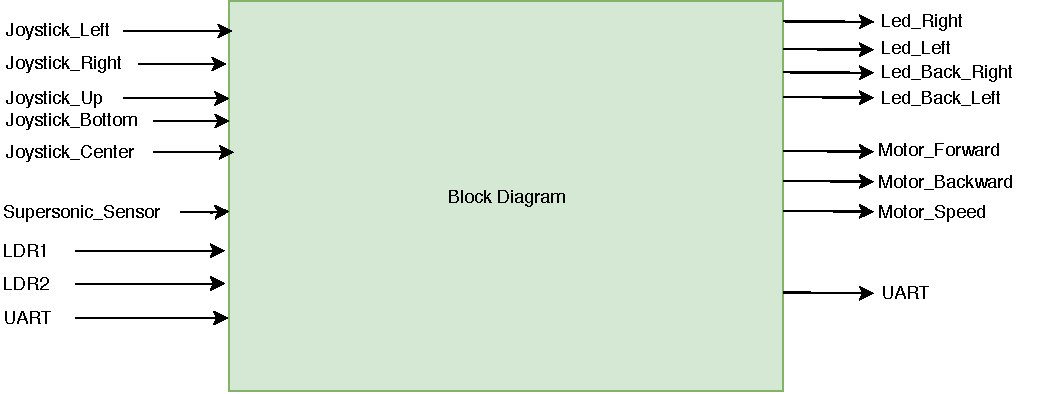
\includegraphics[width=1\columnwidth]{blockdiagram.pdf}
\end{center}
\caption{Block Diagram.}
\vskip\baselineskip % Leave a vertical skip below the figure
\label{fig:sample}
\end{figure}

\newpage
\subsection{Sequence Diagrams}

\begin{figure}[htbp]
\begin{center}
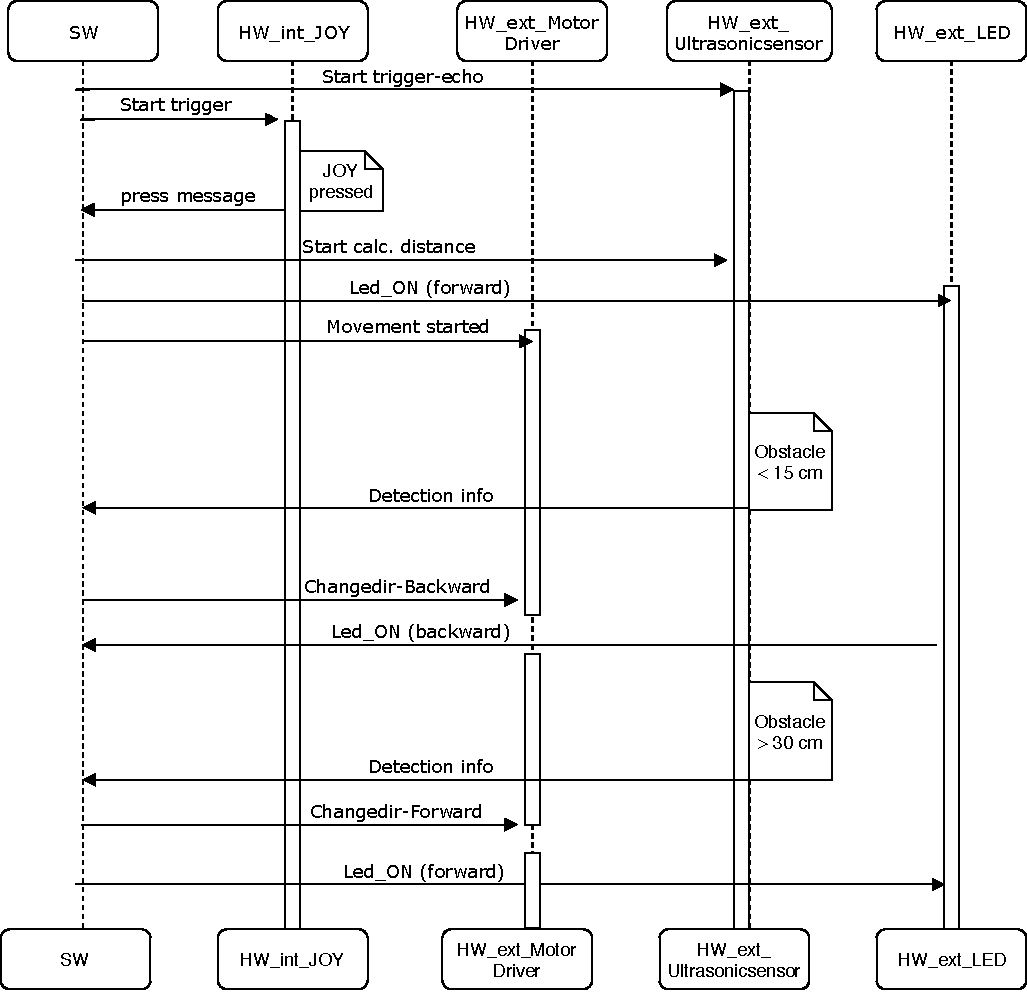
\includegraphics[width=1\columnwidth]{supersonic.pdf}
\end{center}
\caption{Ultrasonic Sequence Diagram.}
\vskip\baselineskip % Leave a vertical skip below the figure
\label{fig:sample}
\end{figure}

\begin{figure}[htbp]
\begin{center}
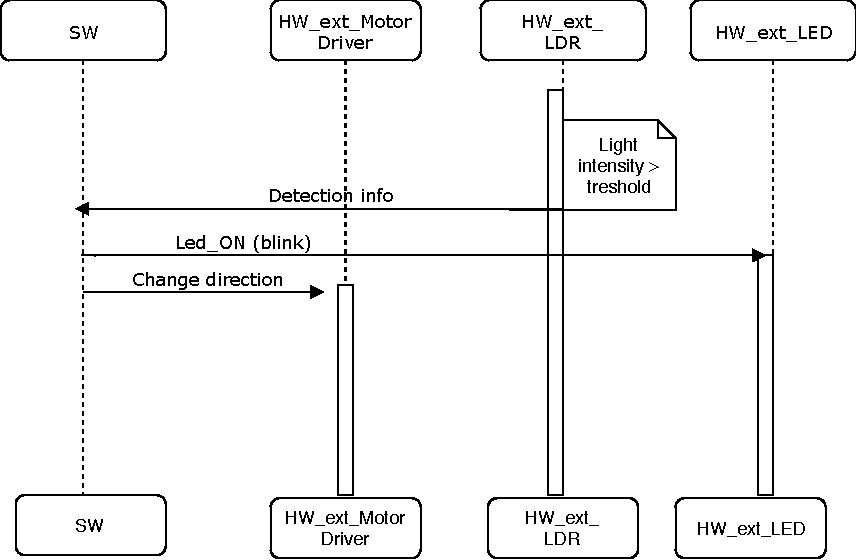
\includegraphics[width=1\columnwidth]{LDR.pdf}
\end{center}
\caption{LDR Sequence Diagram.}
\vskip\baselineskip % Leave a vertical skip below the figure
\label{fig:sample}
\end{figure}

\begin{figure}[htbp]
\begin{center}
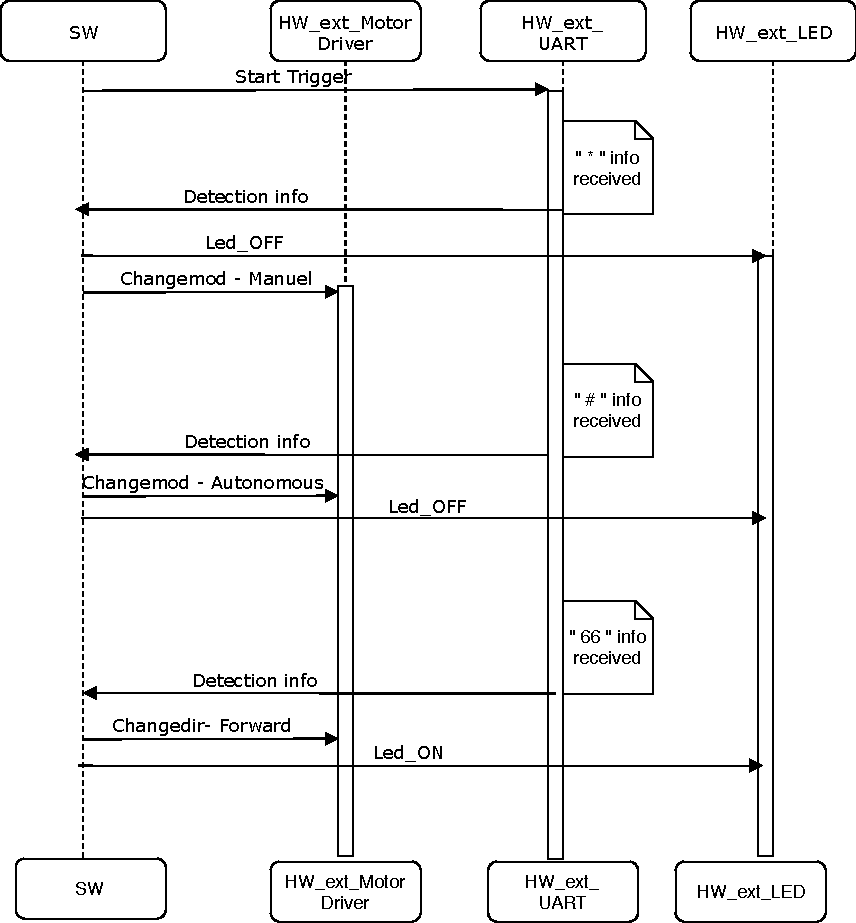
\includegraphics[width=1\columnwidth]{UART.pdf}
\end{center}
\caption{UART Sequence Diagram.}
\vskip\baselineskip % Leave a vertical skip below the figure
\label{fig:sample}
\end{figure}

\newpage
\section{Connections}

\subsection{LED Connections}

Pin functionality is GPIO for each pin. We chose those pins because we just needed a simple GPIO pin without any interference with Joystick and PWM.
\begin {table}[H]
\begin{center}
\begin{tabular}{|c|c|} \hline 
\textbf{LED Pins} & \textbf{LPC4088 Pins} \\ 
\hline 
Led\_Front\_Left & P6 (P1\_23) \\ \hline 
Led\_Front\_Right & P12 (P0\_8) \\ \hline 
Led\_Back\_Left & P5 (P1\_24) \\ \hline 
Led\_Back\_Right & P13 (P0\_7)  \\ \hline 
\end{tabular}
\end{center}
\caption {LED Connection}
\end {table}


\newpage
\subsection{Motor - Driver Connection}
\begin{figure}[htbp]
\begin{center}
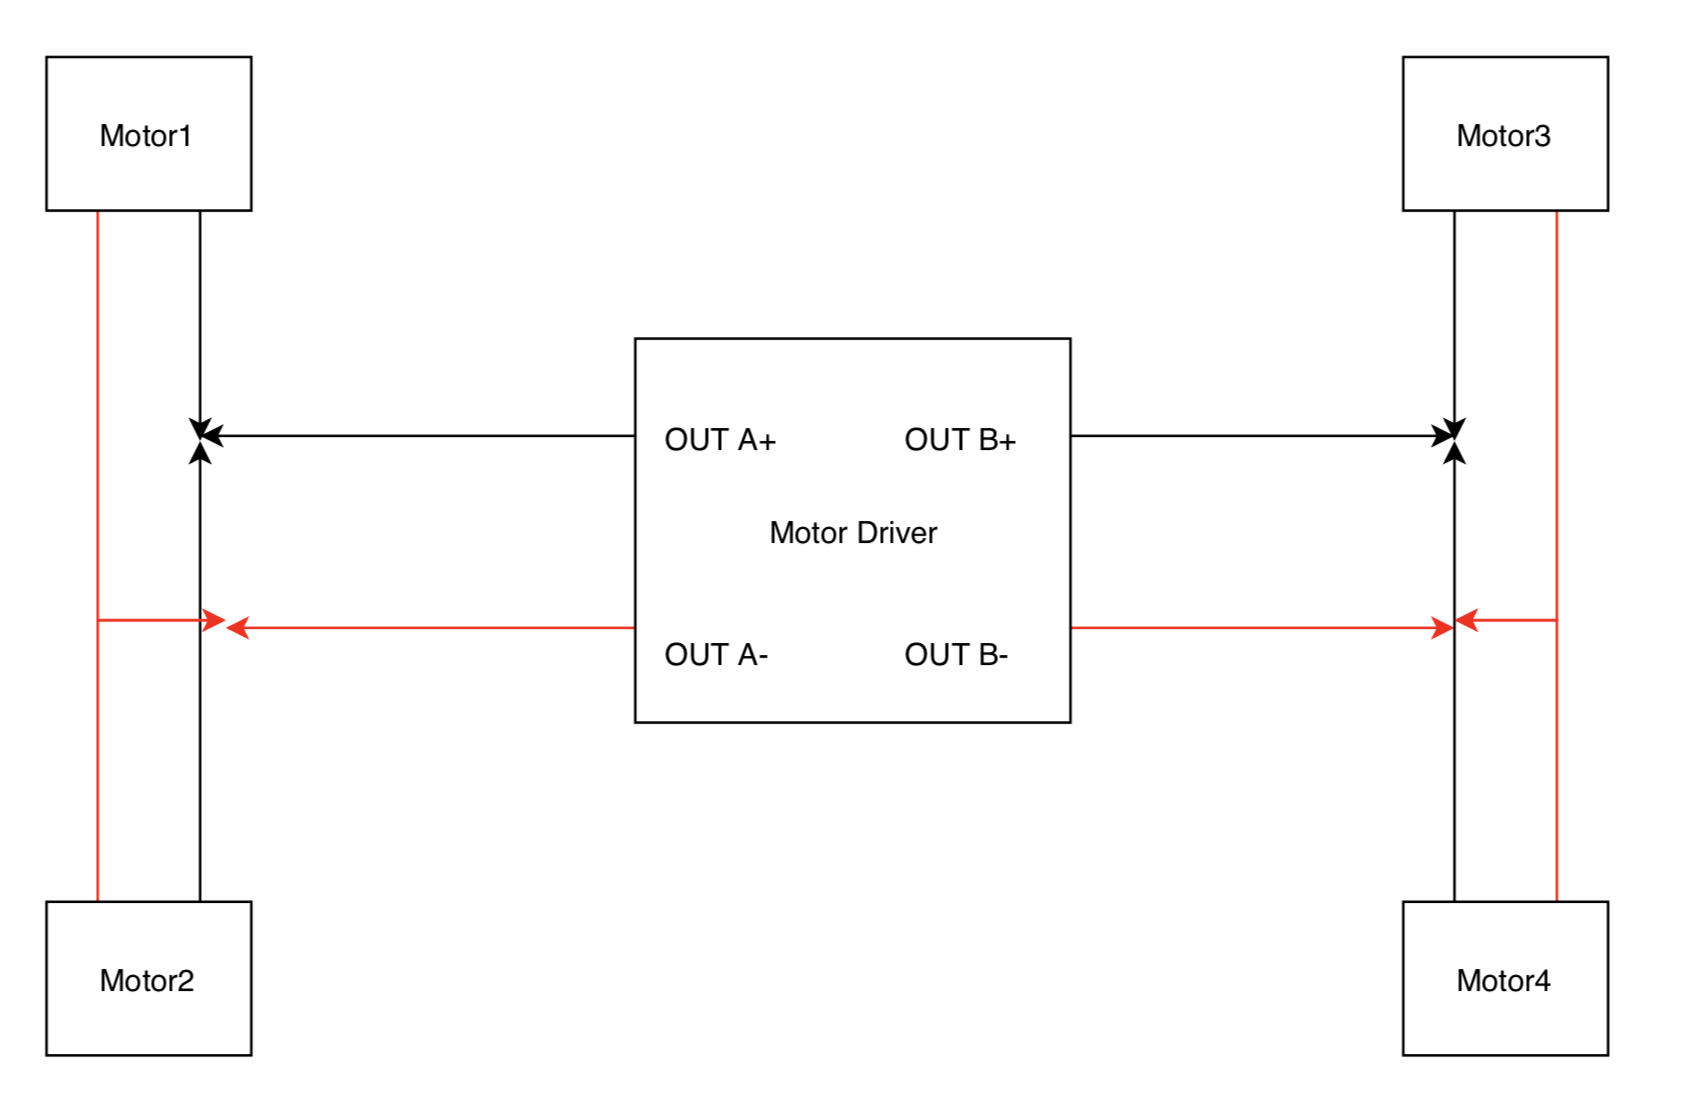
\includegraphics[width=1\columnwidth]{motor.png}
\end{center}
\caption{Motor Driver Connection.}
\vskip\baselineskip % Leave a vertical skip below the figure
\label{fig:sample}
\end{figure}

\newpage
\subsection{Driver - Board Connection}
\begin {table}[H]
\begin{center}
\begin{tabular}{|c|c|} \hline 
\textbf{Motor Controller Pins} & \textbf{LPC4088 Pins} \\ 
\hline 
ENA & P29  \\ \hline 
ENB & P7  \\ \hline 
IN1 & P24  \\ \hline 
IN2 & P19  \\ \hline 
IN3 & P25  \\ \hline 
IN4 & P33  \\ \hline 
\end{tabular}
\end{center}
\caption {Driver-Board Connection}
\end {table}

\subsection{Trimpot Connection}
\begin {table}[H]
\begin{center}
\begin{tabular}{|c|c|c|} \hline 
\textbf{Trimpot Pin} & \textbf{LPC4088 Pins}  & \textbf{ Functionality}\\ 
\hline 
Trimpot & P15 &  001 \\ \hline 
\end{tabular}
\end{center}
\caption {Trimpot Connection}
\end {table}

\subsection{Ultrasonic Sensor Connection}
\begin {table}[H]
\begin{center}
\begin{tabular}{|c|c|c|} \hline 
\textbf{Ultrasonic Pins} & \textbf{LPC4088 Pins} & \textbf{Functionality} \\ 
\hline 
Trigger & P11 & 011  \\ \hline 
Echo & P16 & 011 \\ \hline 
\end{tabular}
\end{center}
\caption {Ultrasonic Sensor Connection}
\end {table}

\subsection{LDR Connection}
\begin {table}[H]
\begin{center}
\begin{tabular}{|c|c|c|} \hline 
\textbf{LDR Pins} & \textbf{LPC4088 Pins} & \textbf{Functionality} \\ 
\hline 
LDR1 & P17 & 001  \\ \hline 
LDR2 & P18 & 001 \\ \hline 
\end{tabular}
\end{center}
\caption {LDR Connection}
\end {table}

\subsection{Push Button Connection}
\begin {table}[H]
\begin{center}
\begin{tabular}{|c|c|c|} \hline 
\textbf{Push Button Pins} & \textbf{LPC4088 Pins} & \textbf{Functionality} \\ 
\hline 
Push Button & P23 & 001  \\ \hline 
\end{tabular}
\end{center}
\caption {Push Button Connection}
\end {table}
\newpage
\section{Circuit Schematics}
\subsection{Led Circuit}
\begin{figure}[!htbp]
\begin{center}
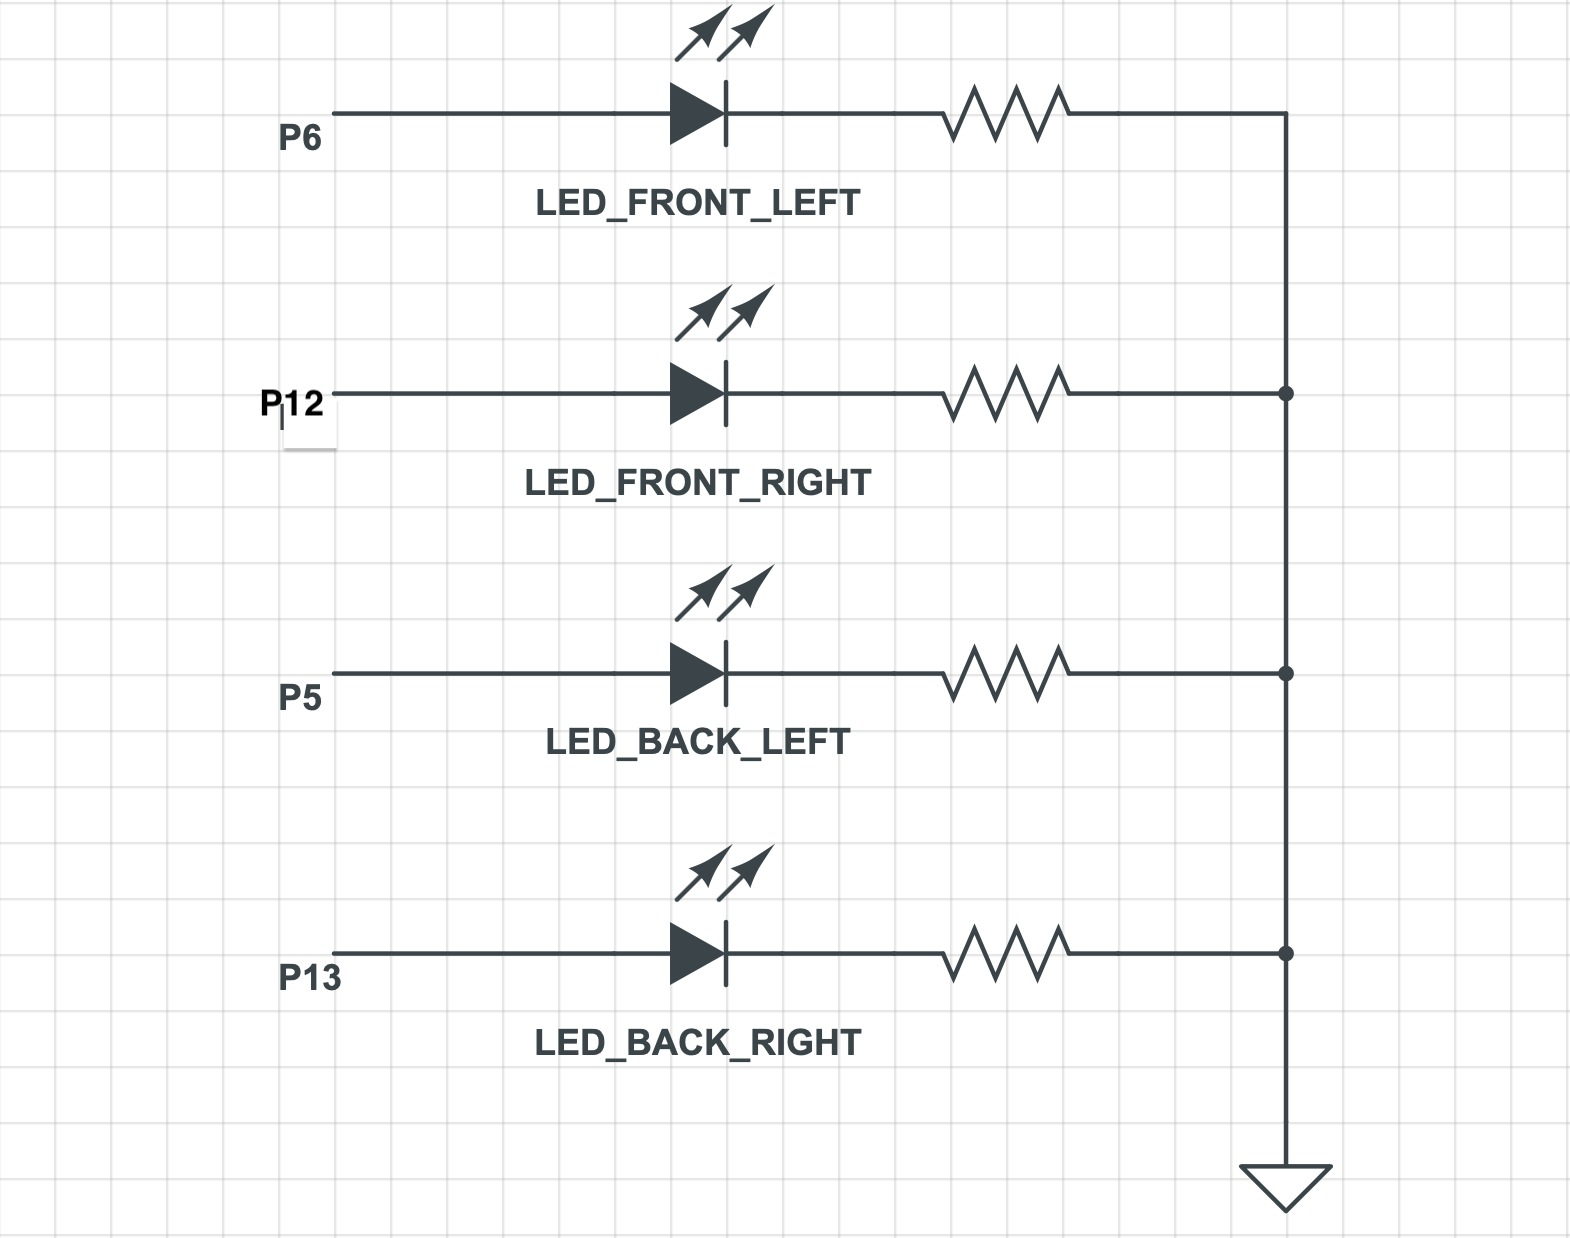
\includegraphics[width=1\columnwidth]{LED.jpeg}
\end{center}
\caption{Led Circuit.}
\vskip\baselineskip % Leave a vertical skip below the figure
\label{fig:sample}
\end{figure}


\newpage
\subsection{LDR Circuit}
\begin{figure}[!htbp]
\begin{center}
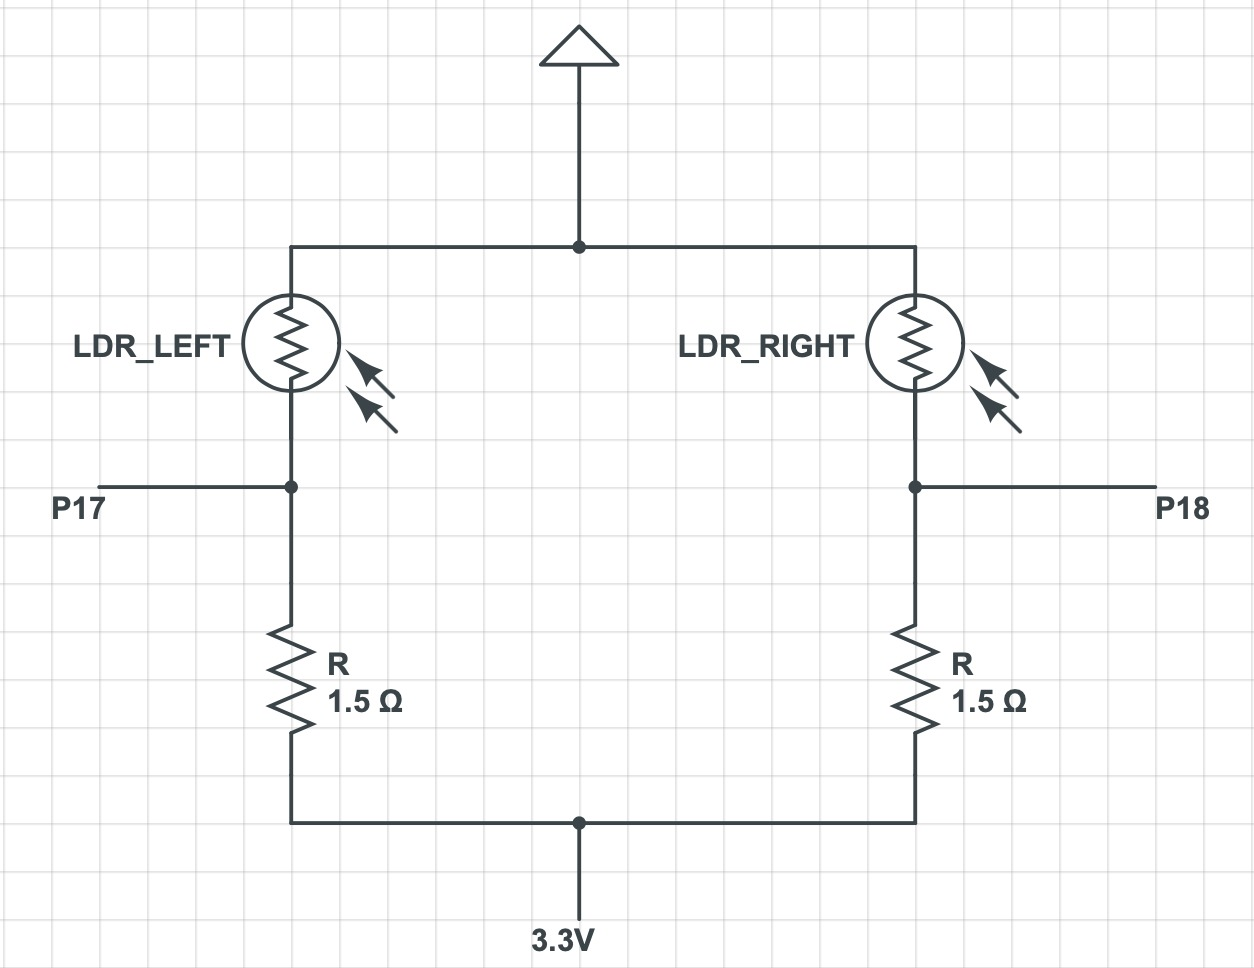
\includegraphics[width=1\columnwidth]{LDR.jpeg}
\end{center}
\caption{LDR Circuit.}
\vskip\baselineskip % Leave a vertical skip below the figure
\label{fig:sample}
\end{figure}
\section{Expense List}
We don't have additional expence.
\newpage
\section{Pseudo Code}

\lstinputlisting[language=C]{code.txt}

\end{document}
%
% End of fbeman.tex
